\chapter{Optimization of \protect\\ Falling and Landing Motions}

This section describes algorithms for generating natural and safe
falling and landing motions of virtual and real humanoids.
In the prior project, we developed an online algorithm for simulated 
characters to generate natural falling and landing motions from 
different heights and initial conditions, while absorbing impact.
In addition, we investigate a scenario of safe falling 
strategy for robots to protect themselves from large external 
perturbations by executing breakfall techniques.

\section{Prior Work: Falling and Landing Motion Control for Character Animation}

\begin{figure}[htbp]
\center
  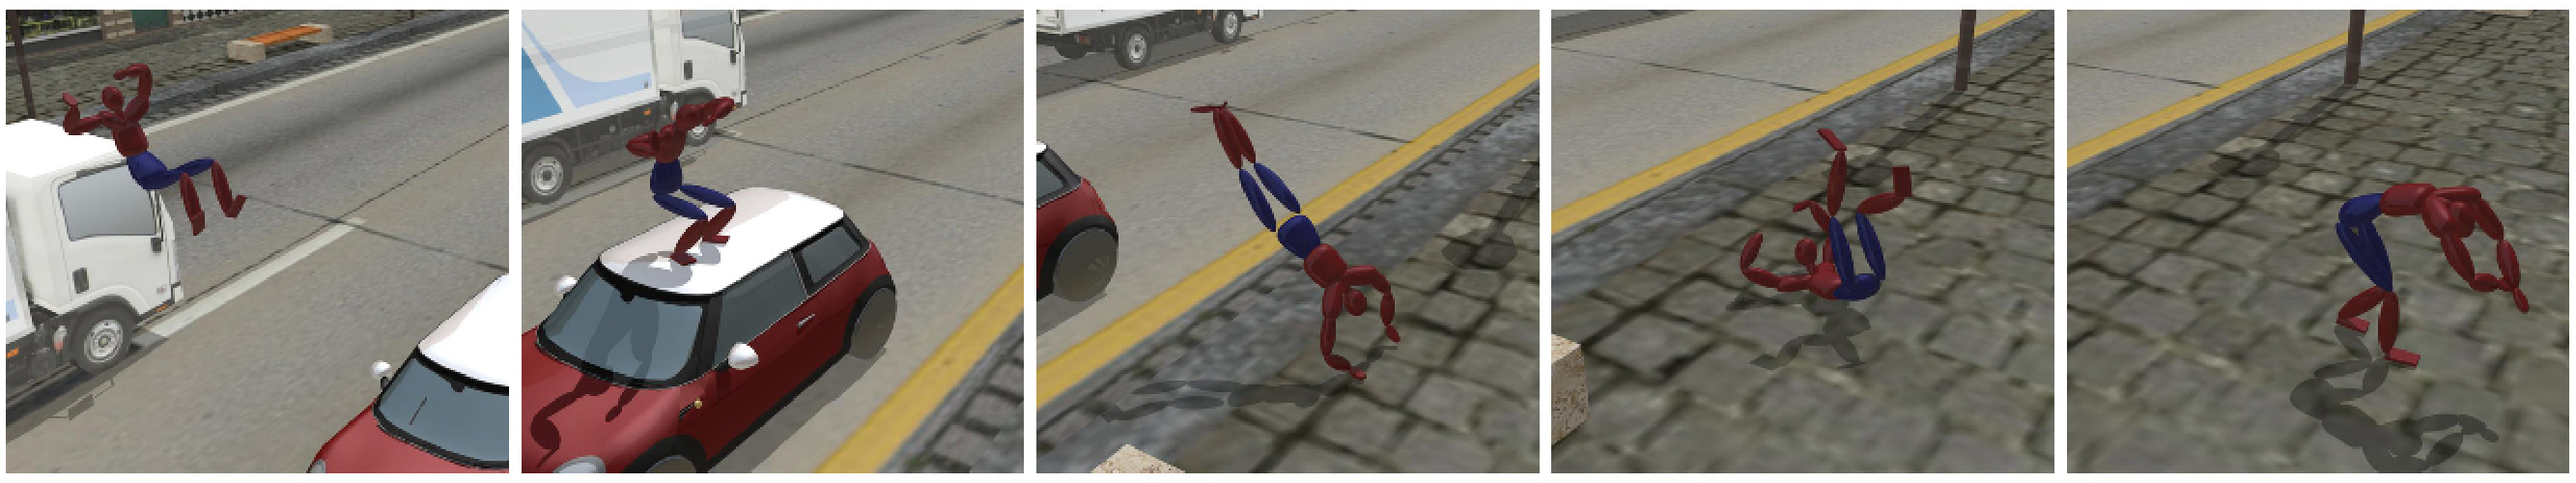
\includegraphics[width=\linewidth]{images/falling1_teaser}
  \caption{A simulated character lands on the roof of a car, 
    leaps forward, dive-rolls on the sidewalk, 
    and gets back on its feet, all in one continuous motion.}
 \label{fig:landingOverview}
\end{figure}

In our prior work \cite{Ha:2012:FAL}, 
we introduce a new method to generate agile and natural human landing
motions in real-time via physical simulation without using any mocap
or pre-scripted sequences. We develop a general controller that allows
the character to fall from a wide range of heights and initial speeds,
continuously roll on the ground, and get back on its feet, without
inducing large stress on joints at any moment 
(\figref{landingOverview}).
The character's motion
is generated through a forward simulator and a control algorithm that
consists of an airborne phase and a landing phase. During the airborne
phase, the character optimizes its moment of inertia to meet the ideal
relation between the landing velocity and the angle of attack, under
the laws of conservation of momentum. The landing phase can be divided
into three stages: impact, rolling, and getting-up. To reduce joint
stress at landing, the character leverages contact forces to control
linear momentum and angular momentum, resulting in a rolling motion
which distributes impact over multiple body parts. We demonstrate that
our control algorithm can be applied to a variety of initial
conditions with different falling heights, orientations, and linear
and angular velocities. Simulated results show that our algorithm can
effectively create realistic action sequences comparable to real world
footage of experienced freerunners.


\section{Multi-contacts Falling Motion Control for a Humanoid Robot}

\subsection{Problem Description}

In this section, we propose to develop a safe falling controller for 
humanoid robots, which ensures the safety of the robots from the
large external perturbations.
Our approach is using the simulation samples for optimizing the controller
to handle complex changes of contacts from highly dynamic fallings.
By breaking a fall into a sequence of multiple contact, like ``UKEMI'' of Judo,
we expect the robot to endure larger external perturbations.
In addition, our simulation-based algorithm allows us to incorporate
an arbitrary objective function so that we can prioritize the body parts
to be protected.

The development of a safe falling controller requires design decisions
on when to detect the falling and how to evaluate the damages from falling.
In this proposal, we assume that the falling can be easily detected 
by observing acceleration of the center of mass and the 
falling controller will be activated after ?? seconds.
Evaluating the damages from the falling might be an interesting problem
to us, because it will dramatically affect the optimal control policy.
We plan to measure the damages on the bodies and joints
as contact forces and joint constraint forces, which might be
scaled to select more important ones to be protected.
Therefore, the objective function of our opitmization is accumulated body
damages and joint stresses while ignoring the negligible value
under the threshold.

\subsection{Related Work}

Safe falling and landing for bipeds is a topic that
receives broad attention in many disciplines. Robotic researchers are
interested in safe falling from standing height for the purpose of
reducing damages on robots due to accidental falls. Previous work has
applied machine learning techniques to predict falling
\cite{Kalyanakrishnan:2011:LPH}, as well as using an abstract model to
control a safe fall
\cite{Fujiwara:2002:FMC,Fujiwara:2007:OPF,Yun:2009:SFH}. 
In contrast to the related work in robotics, we use simulation samples
with detailed robot models to generate the optimal control policy.
The main advantage of using simulation is that it can capture
complex and arbitrary changes of contacts, which is hard to be 
formulated with an abstract model.
We draw inspiration from kinesiology literature and sport practitioners. 
In particular, the techniques developed in freerunning and parkour 
community are of paramount importance for designing landing control 
algorithms capable of handling arbitrary scenarios
\cite{Edwardes:2009:TPF,HLJ:2011:URL}. 

\subsection{Algorithm}

\paragraph{Optimal control for a single scenario}

As the simplified version of the problem, we first develop the falling
controll for a single scenario, which starts from the given initial 
state.
For instance, the robot starts from its initial standing pose and 
being push its head backward for 0.1 second with 10N force.
When we know the parameterization of the controller, optimizing
control parameters for the given scenario can be easily solved
by various optimization techniques, such as 
Covariance Matrix Adaptation (CMA) \cite{Hansen:2004:CMA}).
After solving one instance of the scenarios, we can use the solution
as the guidance for the rest of the scenarios.

\begin{figure}[htbp]
\center
  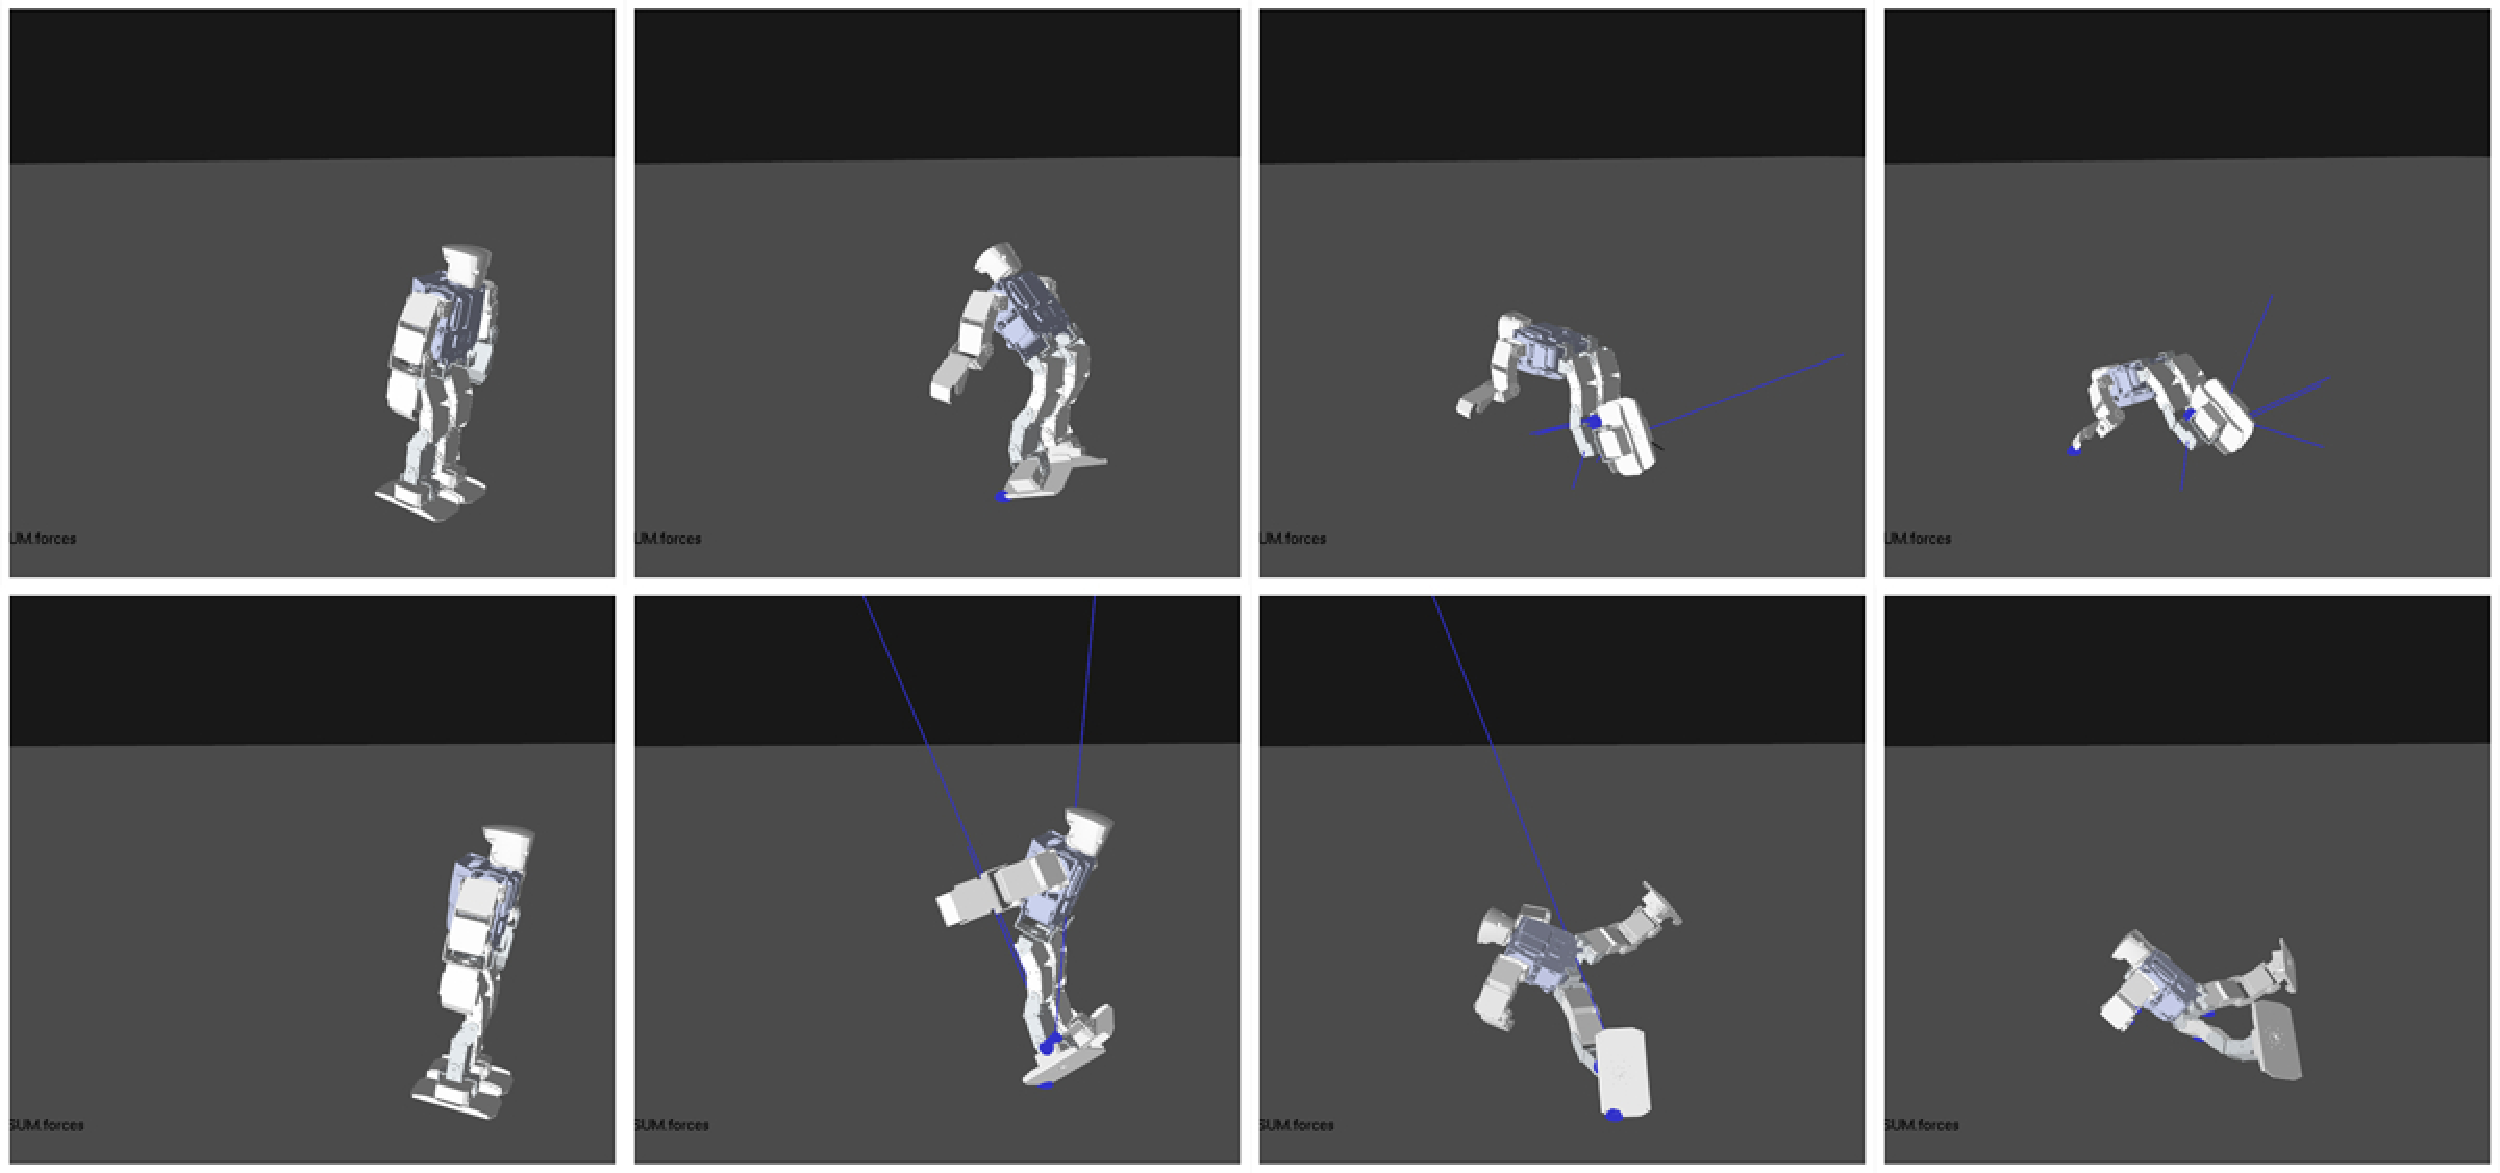
\includegraphics[width=\linewidth]{images/falling2_result}
  \caption{Optimized falling motions with linear joint trajectories (Top)
    and bezier trajectories (Bottom)}

 \label{fig:robotFalling}
\end{figure}

However, finding the proper parameterization of the controller
is a very difficult problem which usually requires a lot of prior knowledge.
In fact, there exist numerous control options in robotics, such as
pose control, torque control, virtual force control using Jacobian
Transpose, and so on.
Even one of the option, a pose control has an infinite number of choices for
representing its joint trajectories with splines.
Indeed, the selection of control dimension has a huge impact on the
result: we tested two parameterization of controller: a pose tracking 
with linear segments and bezier curves, which the latter has four times
more degrees of freedom than the former.
The optimization indicates that the bezier curve gives us 
much better results, which is one third of maximum impact
comparing to the linear control (\figref{robotFalling}).

Therefore, our short term goal is finding the proper parameterization
of the controller.
One intuition from the previous falling and landing project is
momentum planning can be a simple and robust solution, so finding the 
proper momentum trajectory with an abstract model would be 
a promising approach.
Another potential approach is incrementally finding the control 
parameterization. 
In this approach, we search over the optimal parameterization by 
mutating the control dimension with genetic algorithm.
The value of each control dimension will be determined by solving
the optimization problem with the standard technique, like CMA.


\paragraph{Optimal policy for multiple scenarios}

Even if we have an optimal motion for a single scenario,
it is not sufficient for the protection of real robots.
First, the state of the robot is keep changing due to its original
task (i.e. locomotion or manipulation), so we cannot assume
the fixed initial state.
In addition, we may not know the exact information on the current
situation, such as the amount of external forces, because sensors
provides us only limited amount of data that currupted by noise.
Therefore, the optimal motion for the single scenario is not likely 
to be optimal for other situations, and further cause the severe damages
on the body.
To overcome this issue, we need to generate the general policy which 
can react to the sensor data and update the falling motion of the robot.

However, generating an optimal policy is a difficult problem which
requires a lot of samples.
One promising approach is reinforcement learning which optimizes
the best action for the current state by incorporating the long-term
rewards, which is proven to be effective both in computer graphics
\cite{Coros:2009:RTC} and robotics \cite{Morimoto:2004:SRL}.
However, reinforcment learning requires us to select the proper set
of state variables which is still challenging.
If the number of state variables are too many, 
the number of state becomes exponential.
In opposite case, the state variables does not well reflect the 
details of the full-scale simulation.
One possible direction is to use an abstract model such as the 
inverted pendulum (IP) to represent the state in reinforcement learning,
which needs the further investigation and experiments.

\subsection{Expected Results}

\begin{figure}[htbp]
\center
  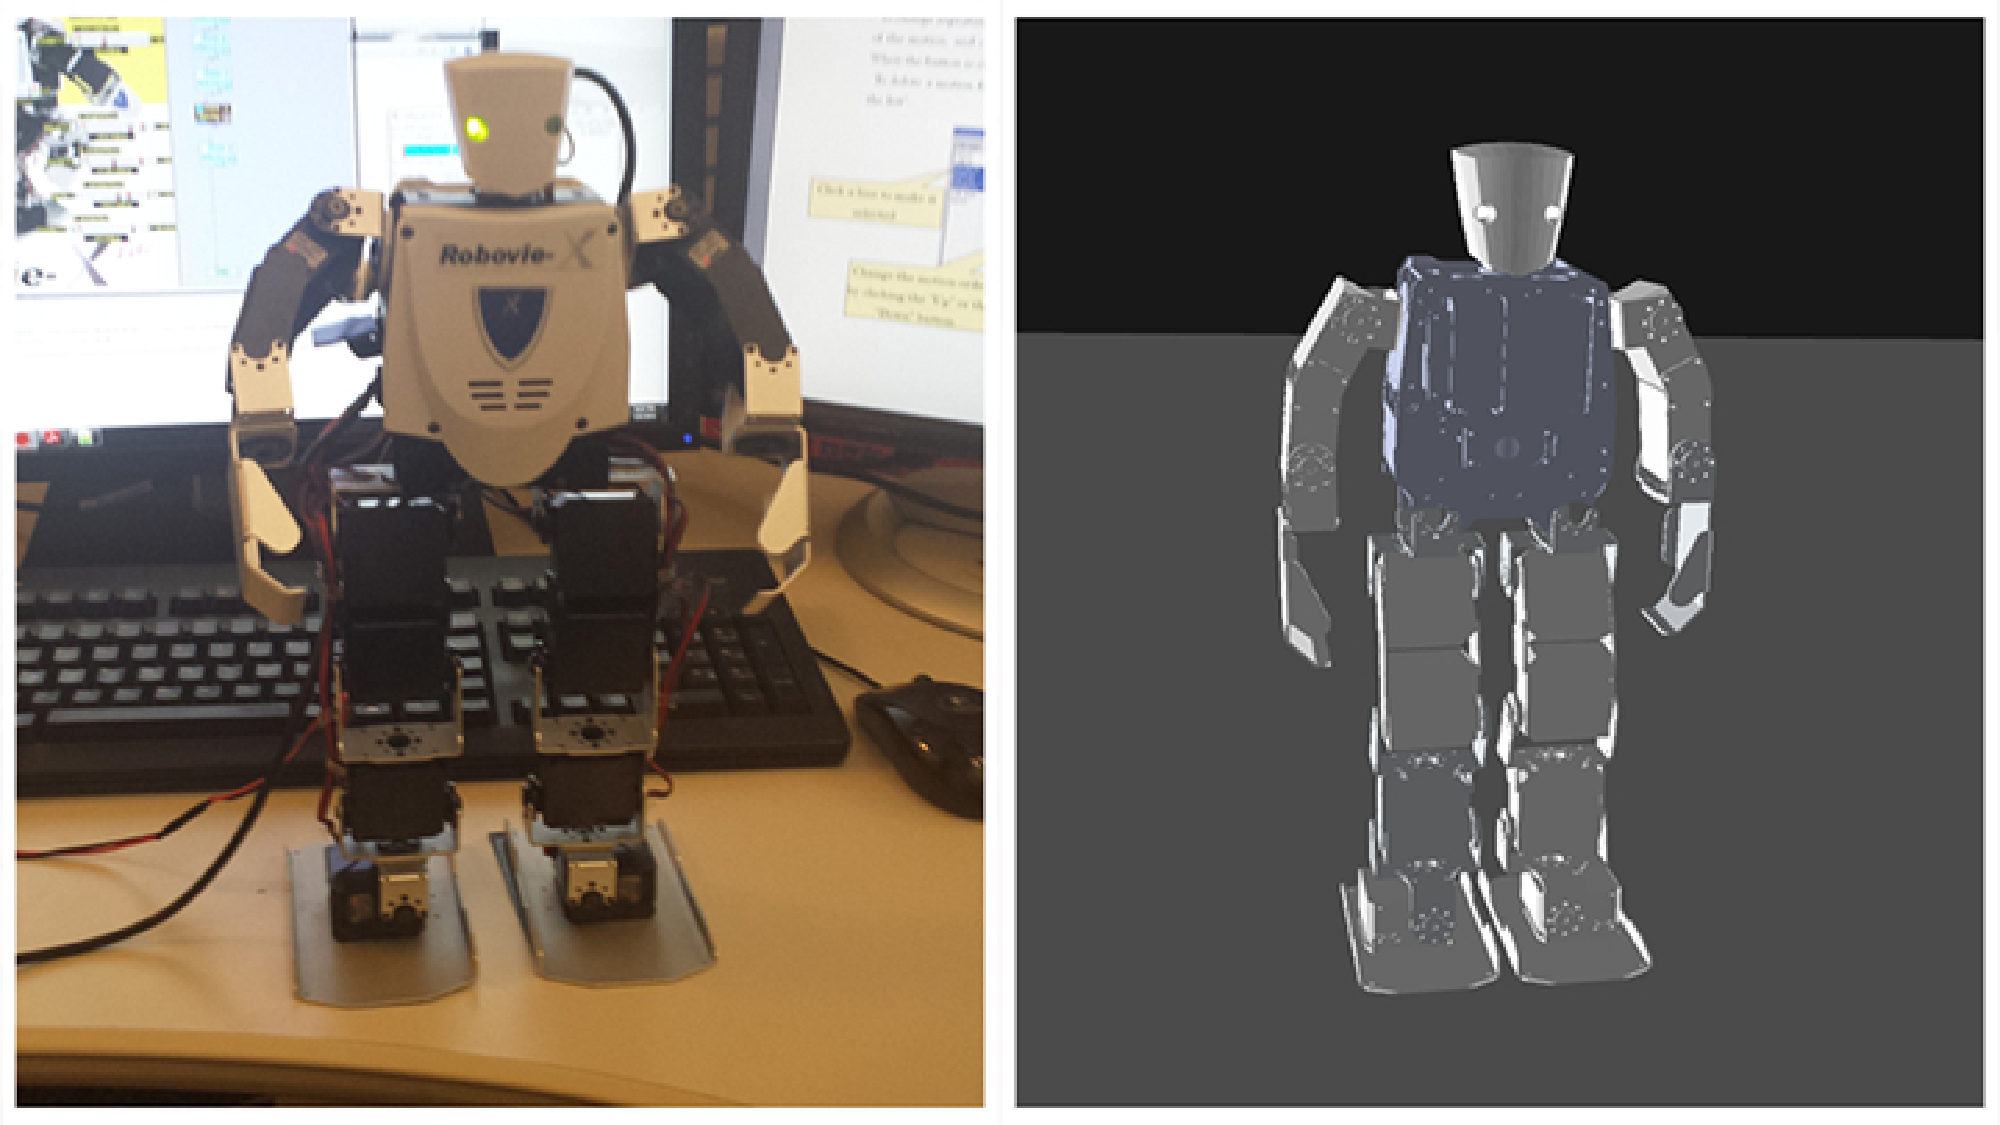
\includegraphics[width=4.2in]{images/falling2_robovies}
  \caption{Real and virtual robovies (Left and Right)} 
 \label{fig:robovies}
\end{figure}

In this project, we try to control safe falling of virtual and real robots
which minimizes the damages on the body parts and joints.
As a testbed, we select a Robovie-X Standard \cite{Robovie} as a target robot
(\figref{robovies}).
A robovie has 17 Degrees of Freedom (Head: 1, Arm: 6, leg 10) 
that are operated by VS-S092J servo motors and a gyro/acceleration sensor board.
The control of robovie is done by their own software, RobovieMaker, 
which takes keyframed trajectories as inputs.
However, we have a plan to change the control framework using Arduino 
for more flexible control.
Moreover, we prepare the virtual model of the robovie from the CAD model,
which can be simulated in Dart simulator \cite{Dart} (\figref{robovies}).
Then the simulation parameters such as torque limit or maximum speeds are 
specified from the specification of servos.

We want to generate a robust falling controller which can handle
a wide range of initial states and external perturbations.
It may include the different state of the robot, different environments, 
and different directions/strengths of pushes.
For all cases, the damage should be minimized which can be verified by 
analyzing the simulation data or the motion captured data of robots.
Further, we will experiment the objective function with user-specified constraints, 
such as "head should be protected" and see how the strategy will be changed.




